\documentclass[tikz,border=5pt]{standalone}
\usepackage{times}
\usepackage{amsmath,amssymb}
\usetikzlibrary{positioning,fit,arrows.meta,backgrounds,shapes.geometric,calc,shadows,decorations.pathreplacing}

\begin{document}
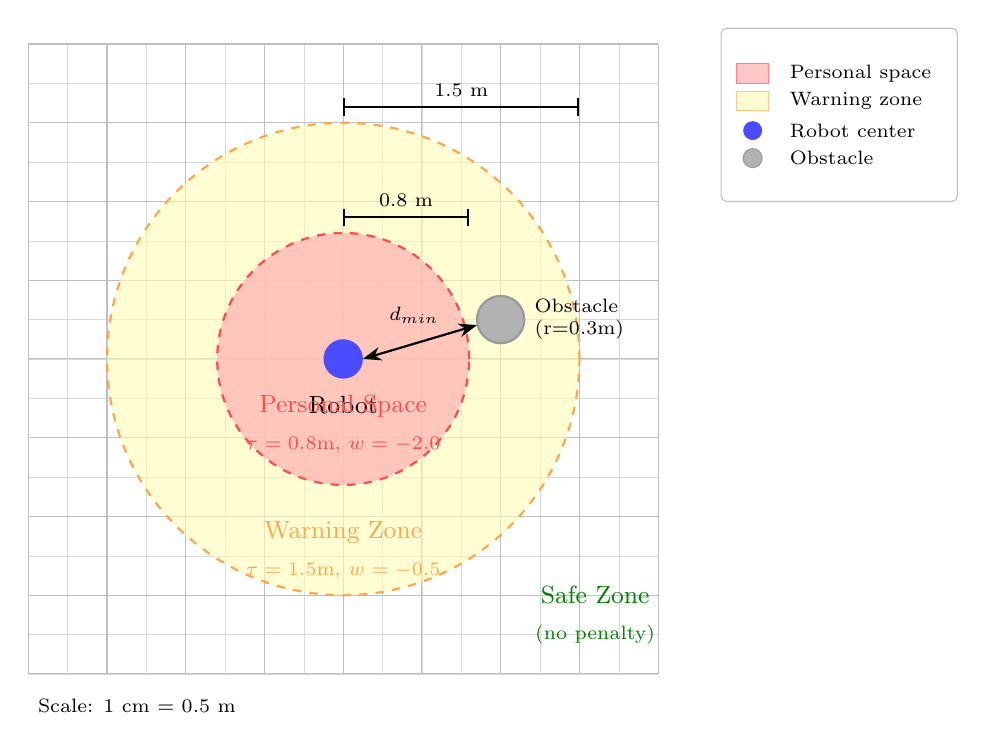
\begin{tikzpicture}[
    scale=1.0,
    label/.style={font=\scriptsize},
    zone_label/.style={font=\small, align=center}
]

% Grid for scale reference
\draw[gray!30, very thin, step=0.5cm] (-4,-4) grid (4,4);
\draw[gray!50, thin, step=1cm] (-4,-4) grid (4,4);

% Warning zone (1.5m radius) - outer yellow zone
\fill[yellow!30, opacity=0.6] (0,0) circle (3cm);

% Personal space zone (0.8m radius) - inner red zone
\fill[red!30, opacity=0.7] (0,0) circle (1.6cm);

% Robot at center
\fill[blue!70] (0,0) circle (0.25cm);
\node[below=0.35cm of {(0,0)}, zone_label] {Robot};

% Zone boundary circles (dashed)
\draw[red!70, dashed, thick] (0,0) circle (1.6cm);
\draw[orange!70, dashed, thick] (0,0) circle (3cm);

% Obstacle cylinder at ~1.0m (within warning zone)
\fill[gray!60] (2.0, 0.5) circle (0.3cm);
\draw[gray!80, thick] (2.0, 0.5) circle (0.3cm);
\node[font=\scriptsize, align=left] at (3.0, 0.5) {Obstacle\\(r=0.3m)};

% Distance measurement arrow
\draw[{Stealth}-{Stealth}, thick] (0.25, 0) -- (1.7, 0.43);
\node[font=\scriptsize] at (0.9, 0.55) {$d_{min}$};

% Zone labels with penalties
\node[zone_label, text=red!70] at (0, -0.6) {Personal Space};
\node[font=\scriptsize, text=red!70] at (0, -1.1) {$\tau = 0.8$m, $w = -2.0$};
\node[zone_label, text=orange!70] at (0, -2.2) {Warning Zone};
\node[font=\scriptsize, text=orange!70] at (0, -2.7) {$\tau = 1.5$m, $w = -0.5$};

% Radius labels
\draw[|-|, thick] (0, 3.2) -- (3, 3.2) node[midway, above, font=\scriptsize] {1.5 m};
\draw[|-|, thick] (0, 1.8) -- (1.6, 1.8) node[midway, above, font=\scriptsize] {0.8 m};

% Safe zone indication
\node[zone_label, text=green!50!black] at (3.2, -3.0) {Safe Zone};
\node[font=\scriptsize, text=green!50!black] at (3.2, -3.5) {(no penalty)};

% Scale reference
\node[font=\scriptsize, anchor=north west] at (-4, -4.2) {Scale: 1 cm = 0.5 m};

% Legend box with background
\begin{scope}[shift={(5.0, 3.5)}]
% Background rectangle
\fill[white, draw=gray!50, rounded corners=2pt] (-0.2, 0.7) rectangle (2.8, -1.5);
% Title
\node[anchor=north west, font=\small\bfseries] at (0, 0.5) {};
% Personal space
\fill[red!30, opacity=0.7, draw=red!70] (0, 0) rectangle (0.4, 0.25);
\node[anchor=west, font=\scriptsize] at (0.55, 0.125) {Personal space};
% Warning zone
\fill[yellow!30, opacity=0.6, draw=orange!70] (0, -0.35) rectangle (0.4, -0.1);
\node[anchor=west, font=\scriptsize] at (0.55, -0.225) {Warning zone};
% Robot center
\fill[blue!70] (0.2, -0.6) circle (0.12cm);
\node[anchor=west, font=\scriptsize] at (0.55, -0.6) {Robot center};
% Obstacle
\fill[gray!60, draw=gray!80] (0.2, -0.95) circle (0.12cm);
\node[anchor=west, font=\scriptsize] at (0.55, -0.95) {Obstacle};
\end{scope}

\end{tikzpicture}
\end{document}
